\documentclass[handout,notheorems]{beamer}

\usepackage[T2A,T1]{fontenc}
\usepackage[utf8]{inputenc}
\usepackage[english]{babel}

\usepackage{tikz}
\usepackage{amsthm}
\theoremstyle{definition}
\newtheorem*{definition}{\textbf{Definition}}

\hypersetup{unicode=true}

\usetheme{CambridgeUS}

\setbeamercolor{frametitle}{parent=palette primary}

\setbeamercolor{block title}{fg=black,bg=white!60!gray}
\setbeamercolor{block body}{fg=black,bg=white!90!gray}

\setbeamercolor*{author in head/foot}{parent=palette tertiary}
\setbeamercolor*{title in head/foot}{parent=palette secondary}
\setbeamercolor*{date in head/foot}{parent=palette primary}

\setbeamercolor*{section in head/foot}{parent=palette tertiary}
\setbeamercolor*{subsection in head/foot}{parent=palette primary}

\setbeamercolor{title}{bg=red!65!black,fg=white}
\setbeamersize{text margin left=1em,text margin right=1em}

% \AtBeginSection[]
% {
%     \begin{frame}{Table of Contents}
%         \tableofcontents[currentsection,hideothersubsections]
%     \end{frame}
% }

\institute[KNU]{Taras Shevchenko National University of Kyiv}
\author[Skybytskyi~N.~M.]{Skybytskyi Nikita, n.skybytskyi@knu.ua}
\title[UAVRP with Moving Targets]{UAVRP with Moving Targets}
\date{\today}

\begin{document}

\begin{frame}
    \titlepage
\end{frame}

\section{TSP, VRP, and Clustering}

\begin{frame}{Traveling Salesman Problem}
    \begin{itemize}
        \item number of vehicles: one;
        \item combinatorial objects: permutations;
        \item objective function: route length.
    \end{itemize}

    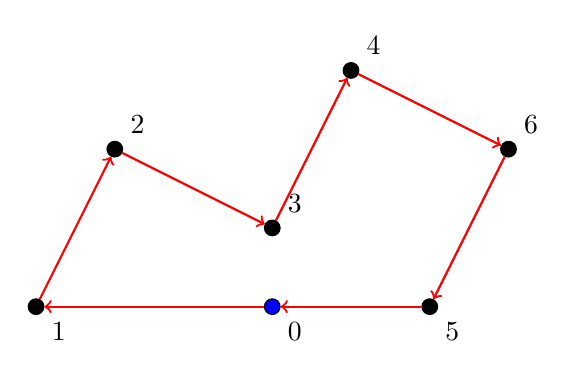
\begin{tikzpicture}[
        point/.style={circle,draw,fill=black,inner sep=2pt},
        edge/.style={->,thick,red}
    ]
        % Define the nodes
        \node[point,label=below right:1] (A) at (0,0) {};
        \node[point,label=above right:2] (B) at (1,2) {};
        \node[point,label=above right:3] (C) at (3,1) {};
        \node[point,label=above right:4] (D) at (4,3) {};
        \node[point,label=below right:5] (E) at (5,0) {};
        \node[point,label=above right:6] (F) at (6,2) {};
        \node[point,fill=blue,label=below right:0] (Depot) at (3,0) {};
        
        % Draw the directed edges and the closed tour
        \draw [edge] (Depot) -- (A);
        \draw [edge] (A) -- (B);
        \draw [edge] (B) -- (C);
        \draw [edge] (C) -- (D);
        \draw [edge] (D) -- (F);
        \draw [edge] (F) -- (E);
        \draw [edge] (E) -- (Depot); % Close the tour
    \end{tikzpicture}
\end{frame}

\begin{frame}{Vehicle Routing Problem}
    \begin{itemize}
        \item number of vehicles: many;
        \item combinatorial objects: partition and permutations;
        \item objective function: sum of route lengths.
    \end{itemize}

    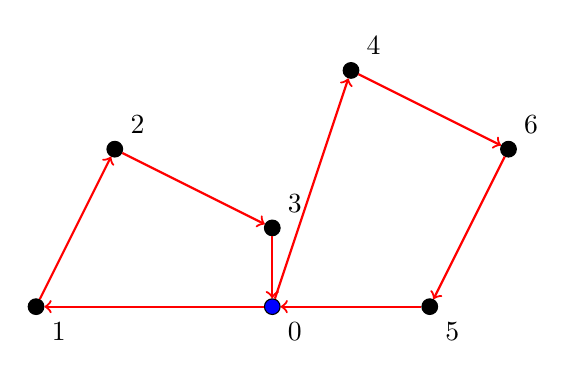
\begin{tikzpicture}[
        point/.style={circle,draw,fill=black,inner sep=2pt},
        edge/.style={->,thick,red}
    ]
        % Define the nodes
        \node[point,label=below right:1] (A) at (0,0) {};
        \node[point,label=above right:2] (B) at (1,2) {};
        \node[point,label=above right:3] (C) at (3,1) {};
        \node[point,label=above right:4] (D) at (4,3) {};
        \node[point,label=below right:5] (E) at (5,0) {};
        \node[point,label=above right:6] (F) at (6,2) {};
        \node[point,fill=blue,label=below right:0] (Depot) at (3,0) {};
        
        % Draw the directed edges and split the tour
        \draw [edge] (Depot) -- (A);
        \draw [edge] (A) -- (B);
        \draw [edge] (B) -- (C);
        \draw [edge] (C) -- (Depot); % Close the tour 1
        
        \draw [edge] (Depot) -- (D);
        \draw [edge] (D) -- (F);
        \draw [edge] (F) -- (E);
        \draw [edge] (E) -- (Depot); % Close the tour 2
    \end{tikzpicture}
\end{frame}

\begin{frame}{Moving Targets}
    Generalizes dynamic depots described in \cite{dynamic-depots}.
    Instead of $x = (x_1, x_2, \ldots, x_d)$ we have $x(t) = f(t)$.
    In the linear case, $x(t) = x_0 + t v$, where $v = (v_1, v_2, \ldots v_d)$. \medskip

    \begin{itemize}
        \item Distance between moving points depends on time (order).
        \item In particular, 2-opt \cite{two-opt} does not apply.
    \end{itemize}
\end{frame}

\begin{frame}{Clustering}
    \begin{itemize}
        \item what: optimal partition;
        \item why: divide and conquer;
        \item how: spacial or temporal proximity.
    \end{itemize}

    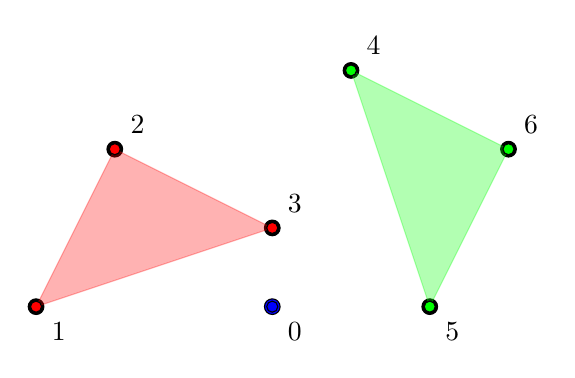
\begin{tikzpicture}[
        point/.style={circle,draw,fill=black,inner sep=2pt},
        edge/.style={->,thick,red}
    ]
        % Define the nodes
        \node[point,label=below right:1] (A) at (0,0) {};
        \node[point,label=above right:2] (B) at (1,2) {};
        \node[point,label=above right:3] (C) at (3,1) {};
        \node[point,label=above right:4] (D) at (4,3) {};
        \node[point,label=below right:5] (E) at (5,0) {};
        \node[point,label=above right:6] (F) at (6,2) {};
        \node[point,fill=blue,label=below right:0] (Depot) at (3,0) {};
    
        % Draw the filled area for the red cluster
        \draw[red,fill=red,opacity=0.3] (A.center) -- (B.center) -- (C.center) -- cycle;
        
        % Draw the filled area for the green cluster
        \draw[green,fill=green,opacity=0.3] (D.center) -- (E.center) -- (F.center) -- cycle;
        
        % Draw the points in clusters
        \draw [point,fill=red] (A) circle (2pt);
        \draw [point,fill=red] (B) circle (2pt);
        \draw [point,fill=red] (C) circle (2pt);
        \draw [point,fill=green] (D) circle (2pt);
        \draw [point,fill=green] (E) circle (2pt);
        \draw [point,fill=green] (F) circle (2pt);
        
        % Draw the depot
        \draw [point,fill=blue] (Depot) circle (2pt);
    \end{tikzpicture}
\end{frame}

\begin{frame}{Two-Level Genetic Algorithm}
    \begin{enumerate}
        \item Clustering moving objects. \cite{moving-clustering}
        \item Find the shortest Hamiltonian \emph{cycle} within each cluster.
        \item Connect cycles between clusters by disconnecting one edge within each cycle.
    \end{enumerate}

    For stationary targets this algorithm was introduced in \cite{tlga}.
\end{frame}

\section{Ordering Power of an Objective Function}

\begin{frame}{Definition of the Ordering Power}
    What is a combinatorial optimization problem?
    \begin{itemize}
        \item a set of meaningful instances $S$;
        \item a finite set of feasible solutions $C = \{c_1, c_2, \dots, c_n\}$ for each $x \in S$;
        \item and an objective function $f: C \to \mathbb{R}$ (wlog $f(c_i) \ne f(c_j)$ for $i \ne j$).
    \end{itemize}
    \pause
    \begin{definition}
        Define a mapping $g: S \to P_n$, where $P_n$ is the set of permutations of $\{1, 2, \dots, n\}$ as follows: $g_i = |\{j: f(c_j(x)) < f(c_i(x))\}|$. In other words, the value of $g$ is an ordering of feasible solutions by the value of the objective function. We call $\log |g(S)|$ an \emph{ordering power of $f$}, as a function of instance size.
    \end{definition}
\end{frame}

\begin{frame}{Example with Classical TSP}
    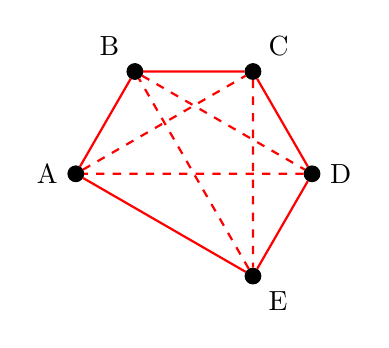
\begin{tikzpicture}[
        point/.style={circle,draw,fill=black,inner sep=2pt},
        edge/.style={thick,gray},
        tour1/.style={thick,red},
        tour2/.style={thick,red,dashed}
    ]
        % Define the nodes
        \node[point,label=left:A] (A) at (180:1.5) {};
        \node[point,label=above left:B] (B) at (120:1.5) {};
        \node[point,label=above right:C] (C) at (60:1.5) {};
        \node[point,label=right:D] (D) at (0:1.5) {};
        \node[point,label=below right:E] (E) at (-60:1.5) {};

        % Highlight the tours
        \draw[tour1] (A) -- (B) -- (C) -- (D) -- (E) -- (A);
        \draw[tour2] (A) -- (C) -- (E) -- (B) -- (D) -- (A);
    \end{tikzpicture}
    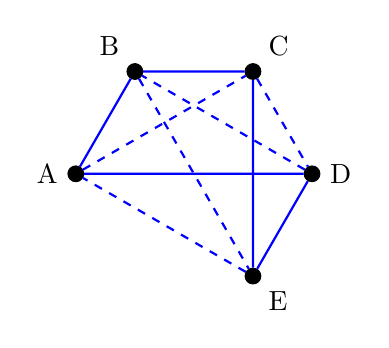
\begin{tikzpicture}[
        point/.style={circle,draw,fill=black,inner sep=2pt},
        edge/.style={thick,gray},
        tour1/.style={thick,blue},
        tour2/.style={thick,blue,dashed}
    ]
        % Define the nodes
        \node[point,label=left:A] (A) at (180:1.5) {};
        \node[point,label=above left:B] (B) at (120:1.5) {};
        \node[point,label=above right:C] (C) at (60:1.5) {};
        \node[point,label=right:D] (D) at (0:1.5) {};
        \node[point,label=below right:E] (E) at (-60:1.5) {};

        % Highlight the tours
        \draw[tour1] (A) -- (B) -- (C) -- (E) -- (D) -- (A);
        \draw[tour2] (A) -- (C) -- (D) -- (B) -- (E) -- (A);
    \end{tikzpicture}
    \pause
    \begin{equation*}
        f(ABCDE) + f(ACEBD) = f(ABCED) + f(ACDBE).
    \end{equation*}
    Therefore, it is impossible to have $f(ABCDE) < f(ABCED)$ and $f(ACEBD) < f(ACDBE)$ simultaneously. The same argument does not hold for moving targets.
\end{frame}

\begin{frame}{Weak Real-Valued Version}
    \begin{definition}
        Define a mapping $g: S \to \mathbb{R}^n$ as follows: $g(x) = (f(c_1(x)), \dots, f(c_n(x)))$. We call $\dim g(S)$ a \emph{weak ordering power of $f$}, as a function of instance size. \textbf{Claim}: the two notions are connected when $g$ is linear.
    \end{definition}
    \pause
    For example, all $n!$ route lengths are continuous functions of $2dn$ variables describing a problem instance with $n$ linearly moving points in $d$-dimensional Euclidean space. Here a point is defined by its position $(x_1, \dots, x_d)$ at time 0 and its velocity $(v_1, \dots, v_d)$. Position of a point at time $t$ is $(x_1 + t v_1, \dots, x_d + t v_d)$. Therefore, $\dim g(S) = 2dn \ll n!$.
\end{frame}

\begin{frame}{}
    \begin{thebibliography}{5}
    \bibitem{dynamic-depots} Horbulin~V.~P., Hulianytskyi~L.~F. and Sergienko~I.~V. Optimization of UAV Team Routes at the Availability of Alternative and Dynamic Depots. \emph{Kibernetyka ta Systemnyi Analiz}. 2020. vol.~56, no.~2. pp.~31--41.
    \bibitem{two-opt} Croes~G.~A. A Method for Solving Traveling-Salesman Problems. \emph{Operations Research}, 1958, vol.~6, no.~6, pp.~791--812.
    \bibitem{moving-clustering} Li~Y. and Han~J., Yang~J. Clustering Moving Objects. \emph{Proceedings of the tenth ACM SIGKDD international conference on Knowledge discovery and data mining}. 2004, pp.~617--622. 
    \bibitem{tlga} Ding,~C., Cheng,~Y. and He,~M. Two-level genetic algorithm for clustered traveling salesman problem with application in large-scale TSPs. \emph{Tsinghua Science \& Technology}, 2007, vol.~12, no.~4, pp.~459--465.
    \bibitem{trig-landing} Savuran~H., Karakaya~M. Route Optimization Method for Unmanned Air Vehicle Launched from a Carrier. \emph{Lecture Notes on Software Engineering}. 2015, vol.~3. pp.~279--284.
    \end{thebibliography}
\end{frame}

\end{document}
